\chapter{Software Project Planning} 
% Main chapter title

\label{Chapter1} 
%Call reference to this chapter use \ref{ChapterX}

\lhead{Chapter 1. \emph{Software Project Planning}} 
% Change X to a consecutive number; this is for the header on each page - perhaps a shortened title

\doublespacing
% LINE FORMATTING

%\clearpage
%\pagebreak

% MAIN SECTION ==============================
\section{Introduction}

\subsection{Project Brief Description}
MTS (My Transportation Schedule) is a daily activity application that could be installed in any Android (An operating system works in mobiles and tablets) device. It focuses on the people who are using the public transportation system in Cyberjaya.\\

The buses among cyberjaya will be provided by a GPS tracker that would track the bus and update the database. The user will be able to organize his timetable through MTS.\\ 

The user is only required to insert the time, the date and location in Cyberjaya of the event, MTS garanties that the user will not be late on any event, by choosing the best route considering the density as well as the traffic. MTS is designed to be able to alarm the user if the target destination cannot be reached on time.

\subsection{MTS is an IoT Software}
Internet of Things (IoT) is a connection of physical objects such as devices, buildings, vehicles, and items embedded through electronics, sensors, softwares, and network connectivity that are allowing all these items to get and exchange data \cite{wikiIOT}.\\

A GPS device is considered as a sensor for tracking the object’s location which is one of the main necessity for an IoT application \cite{second}.\\

Our software uses GPS trackers that are installed to the buses that allows the exchange of data. The software, connects through the GPS with the use of a sim card that allows the GPS to connect to the server that transfers data \cite{third}.\\

\subsection{Project Objectives}
\begin{itemize}
	\item Minimizing the chance of being late. 
	\item Avoid wasting time waiting in the bus station for the bus to come.
	\item Build a software with a good user experience (UX).
\end{itemize}


\pagebreak
%MAIN SECTION ================================
\section{Project Scope}
MTS covers only buses in Cyberjaya. For further prototypes, MTS might be extended to have a wider coverage and more public transportation methods such as trains and Taxis.\\

For starting prototypes, MTS has only four engineers working on it. Which leads to make the starting prototypes used by only few hundreds users to ease the proccess of finding and fixing bugs.\\

For the first prototypes, the application would be bassed on Android operation system. \\

\section{Installation}
MTS needs two servers that are the main server and the backup server to be installed. The backup server will be a copy of the main server. The backup server will be in service automatically if the main server stopped working. Figure \ref{fig:ServerArch} shows the relationship between servers and their databases.

\begin{figure}[H]
	\centering
	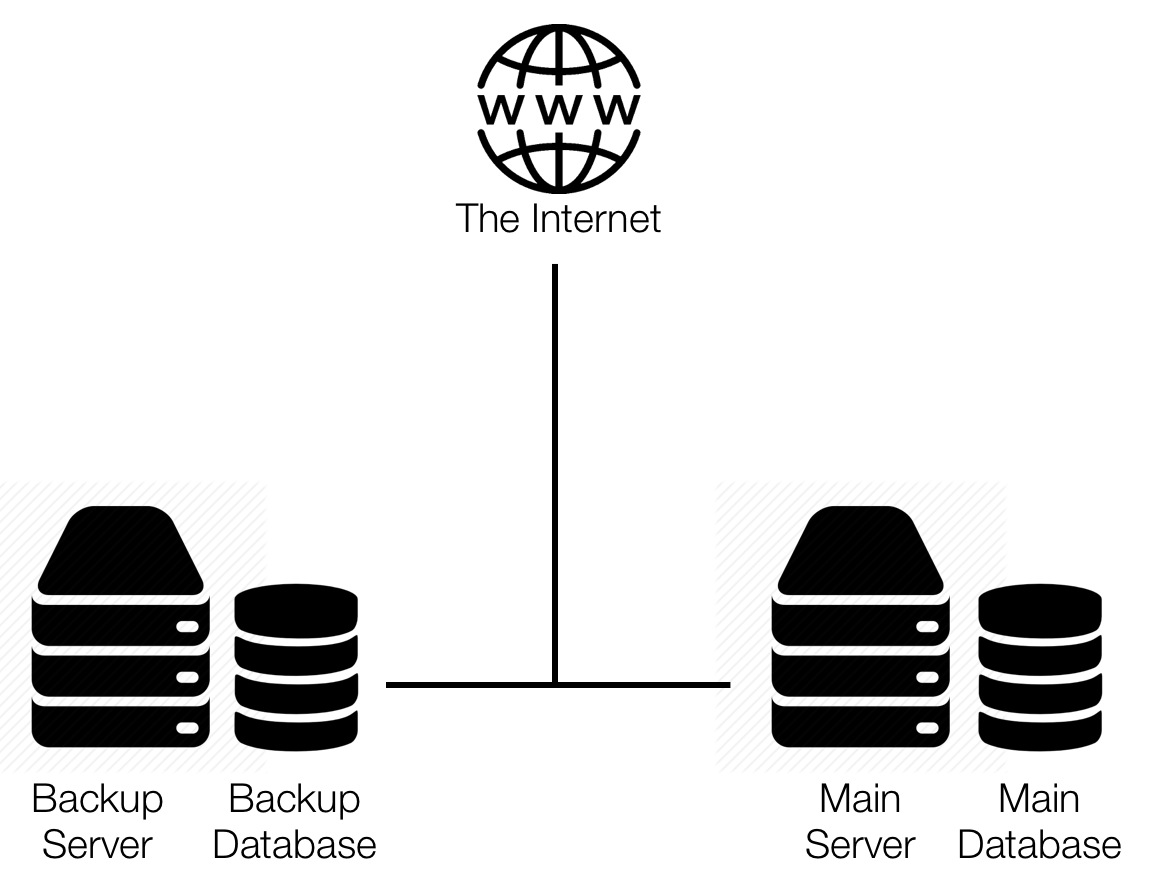
\includegraphics[scale=0.55]{Figures/FigureInstallation.png}
	\rule{35em}{0.5pt}
	\caption[Gantt Chart: Estimated Timeline for a prototype]{Gantt Chart: Estimated Timeline for a prototype}
	\label{fig:ServerArch}
\end{figure}

A chip equipped with a GPS tracker and a SIM card will be installed to every public transportation bus in cyberjaya. The GPS tracker will manage the location tracking function which gets every bus’s location from the GPS  Satellite and update it in the database, while the sim card will be providing the chip with the Internet connection.\\

\section{Execution}
The first two prototypes will be available only for the developers; For the sake of developing and improving. MTS will be available in Google Play after the release of the third prototype. For the ease of testing the prototype, 200 users will be capable of using MTS by then. However, the software will be available for all cyberjaya users after the delivery of the fifth prototype.\\

During execution, feedbacks will be noted from stakeholders in order to list the following prototype’s requirements.


\section{Feedbacks and updates}
At the first two prototypes the developers will list their feedbacks. By the third prototype the users will be able to use and give their feedback about MTS. A feedback is considered as soon as it’s received and the update will be held to the next prototype to be out.



\pagebreak
